\documentclass[journal,12pt,twocolumn]{IEEEtran}

\usepackage{setspace}
\usepackage{gensymb}
\singlespacing
\usepackage[cmex10]{amsmath}

\usepackage{amsthm}

\usepackage{mathrsfs}
\usepackage{txfonts}
\usepackage{stfloats}
\usepackage{bm}
\usepackage{cite}
\usepackage{cases}
\usepackage{subfig}
\DeclareMathAlphabet{\mathpzc}{OT1}{pzc}{m}{it}
\usepackage{longtable}
\usepackage{multirow}
\usepackage{enumitem}
\usepackage{mathtools}
\usepackage{steinmetz}
\usepackage{tikz}
\usepackage{circuitikz}
\usepackage{verbatim}
\usepackage{tfrupee}
\usepackage[breaklinks=true]{hyperref}
\usepackage{graphicx}
\usepackage{tkz-euclide}

\usetikzlibrary{calc,math}
\usepackage{listings}
    \usepackage{color}                                            %%
    \usepackage{array}                                            %%
    \usepackage{longtable}                                        %%
    \usepackage{calc}                                             %%
    \usepackage{multirow}                                         %%
    \usepackage{hhline}                                           %%
    \usepackage{ifthen}                                           %%
    \usepackage{lscape}     
\usepackage{multicol}
\usepackage{chngcntr}

\DeclareMathOperator*{\Res}{Res}

\renewcommand\thesection{\arabic{section}}
\renewcommand\thesubsection{\thesection.\arabic{subsection}}
\renewcommand\thesubsubsection{\thesubsection.\arabic{subsubsection}}

\renewcommand\thesectiondis{\arabic{section}}
\renewcommand\thesubsectiondis{\thesectiondis.\arabic{subsection}}
\renewcommand\thesubsubsectiondis{\thesubsectiondis.\arabic{sub subsection}}


\hyphenation{optical networks semiconduc-tor}
\def\inputGnumericTable{}                                 %%

\lstset{
%language=C,
frame=single, 
breaklines=true,
columns=fullflexible
}
\date{March 2021}

\begin{document}

\newtheorem{theorem}{Theorem}[section]
\newtheorem{problem}{Problem}
\newtheorem{proposition}{Proposition}[section]
\newtheorem{lemma}{Lemma}[section]
\newtheorem{corollary}[theorem]{Corollary}
\newtheorem{example}{Example}[section]
\newtheorem{definition}[problem]{Definition}

\newcommand{\BEQA}{\begin{eqnarray}}
\newcommand{\EEQA}{\end{eqnarray}}
\newcommand{\define}{\stackrel{\triangle}{=}}
\bibliographystyle{IEEEtran}
\raggedbottom
\setlength{\parindent}{0pt}
\providecommand{\mbf}{\mathbf}
\providecommand{\pr}[1]{\ensuremath{\Pr\left(#1\right)}}
\providecommand{\qfunc}[1]{\ensuremath{Q\left(#1\right)}}
\providecommand{\fn}[1]{\ensuremath{f\left({#1}\right)}}
\providecommand{\e}[1]{\ensuremath{E\left(#1\right)}}
\providecommand{\sbrak}[1]{\ensuremath{{}\left[#1\right]}}
\providecommand{\lsbrak}[1]{\ensuremath{{}\left[#1\right.}}
\providecommand{\rsbrak}[1]{\ensuremath{{}\left.#1\right]}}
\providecommand{\brak}[1]{\ensuremath{\left(#1\right)}}
\providecommand{\lbrak}[1]{\ensuremath{\left(#1\right.}}
\providecommand{\rbrak}[1]{\ensuremath{\left.#1\right)}}
\providecommand{\cbrak}[1]{\ensuremath{\left\{#1\right\}}}
\providecommand{\lcbrak}[1]{\ensuremath{\left\{#1\right.}}
\providecommand{\rcbrak}[1]{\ensuremath{\left.#1\right\}}}
\theoremstyle{remark}
\newtheorem{rem}{Remark}
\newcommand{\sgn}{\mathop{\mathrm{sgn}}}
\newcommand{\comb}[2]{{}^{#1}\mathrm{C}_{#2}}
\providecommand{\abs}[1]{\vert#1\vert}
\providecommand{\res}[1]{\Res\displaylimits_{#1}} 
\providecommand{\norm}[1]{\lVert#1\rVert}
%\providecommand{\norm}[1]{\lVert#1\rVert}
\providecommand{\mtx}[1]{\mathbf{#1}}
\providecommand{\mean}[1]{E\sbrak{ #1 }}
\providecommand{\fourier}{\overset{\mathcal{F}}{ \rightleftharpoons}}
%\providecommand{\hilbert}{\overset{\mathcal{H}}{ \rightleftharpoons}}
\providecommand{\system}{\overset{\mathcal{H}}{ \longleftrightarrow}}
	%\newcommand{\solution}[2]{\textbf{Solution:}{#1}}
\newcommand{\solution}{\noindent \textbf{Solution: }}
\newcommand{\cosec}{\,\text{cosec}\,}
\providecommand{\dec}[2]{\ensuremath{\overset{#1}{\underset{#2}{\gtrless}}}}
\newcommand{\myvec}[1]{\ensuremath{\begin{pmatrix}#1\end{pmatrix}}}
\newcommand{\mydet}[1]{\ensuremath{\begin{vmatrix}#1\end{vmatrix}}}
\numberwithin{equation}{subsection}
\makeatletter
\@addtoreset{figure}{problem}
\makeatother
\let\StandardTheFigure\thefigure
\let\vec\mathbf
\vspace{3cm}
\title{EE3900 Gate Assignment - 3}
\author{Adhvik Mani Sai Murarisetty - AI20BTECH11015}
\maketitle
\newpage
\bigskip
\renewcommand{\thetable}{\theenumi}

Download latex-tikz codes from 
%
\begin{lstlisting}
https://github.com/adhvik24/EE3900/blob/main/Gate_A3/main.tex
\end{lstlisting}
%
Download python codes from 
%
\begin{lstlisting}
https://github.com/adhvik24/EE3900/blob/main/Gate_A3/plot.py
\end{lstlisting}
\section{EC 2005/Q.71}
A signal as shown in figure is applied to a matched filter. Which of the following
does represent the output of this matched filter ?
 \begin{figure}[!htp]
\centering
 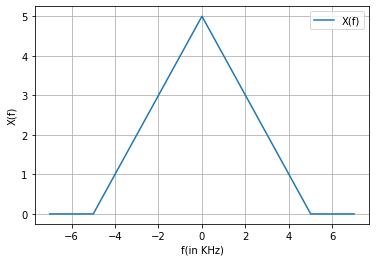
\includegraphics[width=\columnwidth]{0.png}
 \end{figure}

\section{SOLUTION}
\begin{lemma}
    The unit step signal, $u(t)$, is given by:
\begin{align}
    u(t) = 
    \begin{cases}
    1 & t\geq0\\
    0 & otherwise
    \end{cases}
    \label{u(t)}
\end{align}
On time-shifting $u(t)$ by T, we get:
\begin{align}
     u(t - T) =
    \begin{cases}
    1 & t\geq T\\
    0 & otherwise
    \end{cases}
    \label{u(t-T)}
\end{align}
\end{lemma}
\begin{lemma}
Convolution of u(t-a) and u(t-b) is,
\begin{align}
   \nonumber u(t-a)*u(t-b)&=\int\limits_{-\infty}^{\infty}u(\tau-a)u(t-\tau-b) d\tau
\end{align}
\begin{align}
   \nonumber u(t-a)*u(t-b)&= \begin{cases}
    t-b-a & t\geq a+b\\
    0 & otherwise
    \end{cases}
\end{align}
\label{convolve}
\end{lemma}
For a input x(t) the matched filter's impulse response h(t) is,
\begin{align}
    h(t) = x(T-t) \label{0}
\end{align}
The input signal x(t) is,
\begin{align}
    x(t) = u(t)-2u(t-1)+u(t-2)
\end{align}
 \begin{figure}[!htp]
\centering
 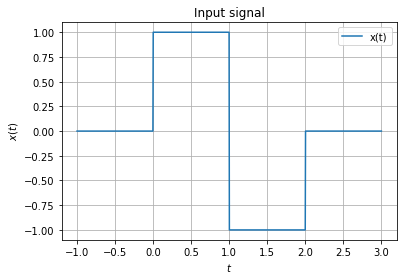
\includegraphics[width=\columnwidth]{input.png}
 \caption{input signal}
 \end{figure}
 
Using \eqref{0}, The impulse response for the matched filter of the input signal is h(t),
\begin{align}
    h(t) = x(2-t)
\end{align}
\begin{align}
    \implies\nonumber h(t) &= x(2-t) = u(2-t)-2u(1-t)+u(-t)\\
\nonumber    \therefore h(t)&= -u(t)+2u(t-1)-u(t-2) = -x(t)
\end{align}
 \begin{figure}[!htp]
\centering
 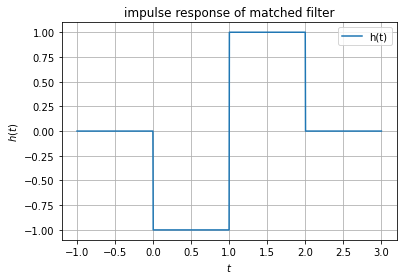
\includegraphics[width=\columnwidth]{h.png}
 \caption{impulse response of matched filter}
 \end{figure}
 
Now, The corresponding output y(t) is given by,
\begin{multline}
    y(t) = h(t) * x(t)\\
    = -(u(t)-2u(t-1)+u(t-2))*\\(u(t)-2u(t-1)+u(t-2))\\
   = -(u(t)*u(t)-4u(t-1)*u(t)+2u(t-2)*u(t))-\\(4u(t-1)*u(t-1)-4u(t-1)*u(t-2))-\\(u(t-2)*u(t-2))
\end{multline}
Using \ref{convolve}, We will get
\begin{align}
    y(t) = \begin{cases}
    0 & t<0\\
    -t & 0\le t < 1\\
    3t-4 & 1\le t <2 \\
    8-3t & 2\le t < 3\\
    t-4 & 3\le t<4\\
    0 & t\ge 4
    \end{cases}
\end{align}
 \begin{figure}[!htp]
\centering
 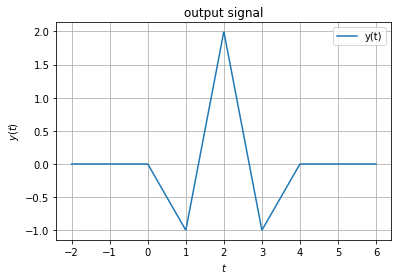
\includegraphics[width=\columnwidth]{output.png}
 \caption{output signal}
 \end{figure}
 \textbf{Therefore, Option(C) is the correct option.}
\end{document}
